\documentclass[tikz]{standalone}
\usetikzlibrary{positioning}
\usepackage{mathtools}

\newcommand{\red}[1]{\textcolor{red}{#1}}
\newcommand{\blue}[1]{\textcolor{blue}{#1}}
\newcommand{\teal}[1]{\textcolor{teal}{#1}}
\newcommand{\hb}{\texttt{hb}}
\newcommand{\vis}{\texttt{vis}}
\newcommand{\so}{\texttt{so}}
\newcommand{\ar}{\texttt{ar}}
\newcommand{\tord}[1]{\textsl{to}(#1)}

\newcommand{\wcc}{\textsl{WCC}}
\newcommand{\wccv}{\textsl{WCCv}}
\newcommand{\cm}{\textsl{CM}}
\newcommand{\cmv}{\textsl{CMv}}
\newcommand{\ccc}{\textsl{CC}}
\newcommand{\ccv}{\textsl{CCv}}
\newcommand{\scc}{\textsl{SCC}}
\newcommand{\sccv}{\textsl{SCCv}}

\begin{document}
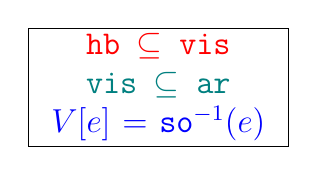
\begin{tikzpicture}
\tikzset{
  lconsistency/.style = {rectangle, fill=white, font=\large, draw, inner sep = 2pt, text width=11em, text centered},
  sconsistency/.style = {rectangle, fill=white, font=\large, draw, inner sep = 2pt, text width=9em, text centered},
  ssconsistency/.style = {rectangle, fill=white, font=\large, draw, inner sep = 2pt, text width=6em, text centered},
  lemma/.style = {rectangle, rounded corners, fill=white, draw=white, line width = 1.5pt, inner sep = 6pt},
  po/.style = {->, very thick},
  cn/.style = {rectangle, fill=white, draw=white,font=\Large},
}

  \node (cc) [sconsistency] {%\large CC\\
                             \red{$\hb \subseteq \vis$}\\
                             \teal{$\vis \subseteq \ar$}\\
                             \blue{$V[e] = \so^{-1}(e)$}};
  %\node (ncc) [cn, below = 0.1cm of cc] {\cm};

\end{tikzpicture}
\end{document}
